\documentclass[11pt,a4paper]{article}

% ================================================================
% Human Design as a Geometric Coding Layer
% Research draft / reproducible manuscript
% Compatible with Visual Studio Code + LaTeX Workshop and Overleaf
% ================================================================

\usepackage[utf8]{inputenc}
\usepackage[T1]{fontenc}
\usepackage{lmodern}
\usepackage[a4paper,margin=2.6cm]{geometry}
\usepackage{microtype}
\usepackage{amsmath,amssymb,amsfonts,mathtools,bm}
\usepackage{booktabs}
\usepackage{array}
\usepackage{multirow}
\usepackage{enumitem}
\usepackage{graphicx}
\usepackage{tikz}
\usetikzlibrary{arrows.meta,positioning,calc,fit,shapes.geometric,decorations.pathreplacing}
\usepackage{xcolor}
\usepackage{url}
\usepackage{natbib}
\usepackage{hyperref}
\usepackage[nameinlink,noabbrev]{cleveref}

\hypersetup{
  colorlinks=true,
  linkcolor=blue!50!black,
  citecolor=green!40!black,
  urlcolor=blue!55!black,
  pdftitle={Human Design as a Geometric Coding Layer},
  pdfauthor={Research draft},
  pdfsubject={64 x 6 x 6 x 6 x 5 geometric information space}
}

\setlength{\parindent}{0pt}
\setlength{\parskip}{0.55em}
\numberwithin{equation}{section}
\newcommand{\R}{\mathbb{R}}
\newcommand{\Z}{\mathbb{Z}}
\newcommand{\F}{\mathbb{F}}
\newcommand{\HH}{\mathcal{H}}
\newcommand{\XX}{\mathcal{X}}
\newcommand{\PP}{\mathcal{P}}
\newcommand{\UU}{\mathcal{U}}
\newcommand{\eps}{\varepsilon}
\newcommand{\rhoP}{\rho}
\newcommand{\tr}{\operatorname{tr}}
\newcommand{\Fix}{\operatorname{Fix}}
\newcommand{\diag}{\operatorname{diag}}
\newcommand{\rank}{\operatorname{rank}}
\newcommand{\Span}{\operatorname{span}}

% Safe figure inclusion: compiles before the raster/vector figures exist.
\newcommand{\safegraphic}[3][]{%
  \IfFileExists{#2}{%
    \includegraphics[#1]{#2}%
  }{%
    \begin{center}
    \fbox{\begin{minipage}[c][#3][c]{0.88\linewidth}
      \centering\small
      \textbf{Figure asset pending.}\\[0.35em]
      \texttt{\detokenize{#2}}\\[0.35em]
      Replace this placeholder with the reproducible figure generated by the audit pipeline.
    \end{minipage}}
    \end{center}
  }%
}

\newcommand{\resultstatus}[1]{\textbf{Status: #1}}

\title{\textbf{Human Design as a Geometric Coding Layer:}\\
From the 64 I~Ching Hexagrams to Quasicrystalline Geometry,\\
QVSM Operators, Weyl Certification, and Quantum Correlations}
\author{Research manuscript / reproducible computational draft}
\date{Version 1.0 -- October 2026}

\begin{document}
\maketitle

\begin{abstract}
This manuscript proposes a mathematically explicit framework in which the discrete architecture used by Human Design is treated as a coding layer for a larger geometric information space. The starting coordinates are a Gate/hexagram index, its six Line values, and three deeper sub-structures (Color, Tone, and Base), giving
\[
64\times6\times6\times6\times5=69\,120
\]
canonical states. The number 69,120 is not introduced ad hoc: public Human Design documentation itself describes a 64-fold Gate structure whose Gates are subdivided into six Lines, six Colors, six Tones and five Bases. The present work does not interpret that descriptive claim as evidence for a physical mechanism; instead, it asks whether the discrete architecture can be represented as a reproducible mathematical state space.

The proposed construction proceeds through several layers: a 6-bit hypercube representation of the 64 hexagrams; a $\mathbb Z_2$ complement involution; linear projection to three-dimensional geometric sectors; a $64\times3=192$ tensor-product lifting associated with a $T_2/T_{2u}$-type representation; a quasicrystalline cut-and-project embedding; a supergolden substitution with Perron root $\psi$ satisfying $\psi^3-\psi^2-1=0$; a factored quantum-vector-state model (QVSM); and a Weyl/Merkle audit layer (PRISM/QWLP) intended to certify transformations and invariants. The manuscript also places the framework next to modern measurements of quantum correlations in $H\to ZZ^*\to4\ell$, while explicitly rejecting any inference that Human Design itself has thereby been physically validated.

The main scientific objective is therefore methodological: to determine which correspondences survive exact algebra, independent numerical reproduction, group-theoretic auditing, and eventually experiment. We separate established mathematics, computational results generated by the project, and conjectural physical interpretations so that future tests can falsify the latter without weakening the former.
\end{abstract}

\textbf{Keywords:} Human Design; I~Ching; hypercube; cut-and-project; quasicrystal; supergolden ratio; $T_{2u}$; quantum information; Bell correlations; Weyl group; Merkle audit; reproducibility.

\tableofcontents
\newpage

% ================================================================
\section{Scope, claims, and epistemic status}
\label{sec:scope}

The central proposal is deliberately narrower than a claim that Human Design is a physical theory. We treat Human Design as a \emph{symbolic/discrete input language} and ask whether its internal combinatorial architecture can be embedded into a mathematically controlled geometry.

Three evidence levels are used throughout:

\begin{enumerate}[label=\textbf{L\arabic*.},leftmargin=2.2em]
  \item \textbf{Established mathematics.} Identities concerning finite sets, hypercubes, group actions, tensor products, spectral radii, projections, density matrices, and cryptographic hash trees.
  \item \textbf{Project computational results.} Results reported by the author's current computational pipeline and to be independently reproduced from the files named in the audit manifest. These are not treated as independently peer-reviewed results merely because a script reproduces them.
  \item \textbf{Hypotheses.} Proposed correspondences connecting the coding space to physical quasicrystals, optical response, matter--antimatter geometric models, or quantum observables.
\end{enumerate}

The distinction is essential. In particular, numerical agreement in an abstract representation does not establish a causal relation between Human Design and a material or quantum system.

% ================================================================
\section{Introduction}
\label{sec:introduction}

Human Design publicly describes its Rave Mandala through a 64-part outer structure derived from the 64 I~Ching hexagrams. Its documentation further describes a Gate substructure in which each Gate is divided into six Lines, six Colors, six Tones and five Bases, yielding 1,080 values per Gate and 69,120 points in the full mandala \,\citep{JovianArchiveBasics2026,JovianArchiveDictionary2026}. The existence of this discrete hierarchy is the starting datum of this manuscript; its metaphysical interpretation is outside the scope of the mathematical derivations.

The remarkable opportunity is that the $64$ layer has a canonical mathematical realization:
\[
64=2^6,
\]
so the set of six-bit words
\[
\HH_6=\{0,1\}^6
\]
contains exactly 64 states. This gives an immediate route from hexagram symbolism to Hamming geometry, graph structure and group actions without assigning a physical meaning to the bits.

The second observation is that the full hierarchy can be indexed in the fixed order
\[
G\rightarrow L\rightarrow C\rightarrow T\rightarrow B,
\]
with
\[
G\in\Z_{64},\quad L,C,T\in\Z_6,\quad B\in\Z_5.
\]
The canonical integer index is
\begin{equation}
 i=((((G\,6+L)\,6+C)\,6+T)\,5+B),
 \qquad 0\le i<69\,120.
\label{eq:canonical-index}
\end{equation}
The order is fixed throughout the paper because a change of factor ordering would define a different coordinate convention.

The resulting research question is:
\begin{quote}
Can the 69,120-point symbolic space be endowed with a hierarchy of geometries and operators whose invariants can be computed exactly, learned, independently audited, and eventually compared with physical data?
\end{quote}

% ================================================================
\section{Human Design as a discrete coding layer}
\label{sec:HD}

\subsection{The 64 Gate/hexagram layer}

Let
\[
G\in\{0,1,\dots,63\}
\]
be the Gate index. We use the standard binary identification only as a mathematical encoding, not as a claim that the six bits are physical degrees of freedom.

The source architecture is documented as 64 hexagrams/Gates with six Lines each \citep{JovianArchiveGates2026}. The deeper subdivision documented by Human Design terminology is
\[
\text{Gate}\rightarrow\text{Line}\rightarrow\text{Color}\rightarrow\text{Tone}\rightarrow\text{Base}.
\]
The corresponding cardinalities are
\[
64,\qquad 6,\qquad 6,\qquad 6,\qquad 5.
\]
Consequently,
\begin{equation}
|\XX|=64\cdot6\cdot6\cdot6\cdot5=69\,120.
\label{eq:69120}
\end{equation}

This reproduces the 69,120-point count described in Human Design's own public documentation \citep{JovianArchiveBasics2026}. The contribution of the present paper is to formalize the same cardinality as a Cartesian state space and then study its transformations.

\subsection{Canonical state space}

Define
\begin{equation}
\XX=\Z_{64}\times\Z_6\times\Z_6\times\Z_6\times\Z_5.
\label{eq:X}
\end{equation}
A state is
\[
X=(G,L,C,T,B).
\]
The product structure is intentionally factored rather than represented as a dense $69,120\times69,120$ matrix. This permits algorithms whose complexity scales with the individual factors.

A translation operator can be defined component-wise by
\begin{equation}
\tau_{\Delta G,\Delta L,\Delta C,\Delta T,\Delta B}
(G,L,C,T,B)
=
(G+\Delta G, L+\Delta L, C+\Delta C,T+\Delta T,B+\Delta B),
\end{equation}
where the additions are taken modulo $(64,6,6,6,5)$ respectively.

% ================================================================
\section{The 64 states as a six-dimensional hypercube}
\label{sec:hypercube}

Represent each Gate/hexagram by a binary vector
\begin{equation}
 g=(g_1,g_2,g_3,g_4,g_5,g_6)\in\{0,1\}^6.
\end{equation}
Then
\[
|\{0,1\}^6|=2^6=64.
\]
The graph with these 64 vertices and edges differing in exactly one bit is the six-dimensional hypercube $Q_6$ \citep{Coxeter1973,Harary1972}.

The natural graph distance is the Hamming distance
\begin{equation}
 d_H(g,g')=\sum_{k=1}^{6}|g_k-g_k'|.
\end{equation}
For the 64 binary states the distance distribution from a fixed vertex is
\[
\binom{6}{0},\binom{6}{1},\binom{6}{2},\binom{6}{3},\binom{6}{4},\binom{6}{5},\binom{6}{6}
=
1,6,15,20,15,6,1.
\]

A particularly simple involution is complementation:
\begin{equation}
 g^c=g\oplus(1,1,1,1,1,1),
\qquad
(g^c)^c=g.
\end{equation}
After centering bits by $\tilde g_i=g_i-1/2$, complementarity becomes
\begin{equation}
 \tilde g_i^c=-\tilde g_i.
\end{equation}
Therefore any linear coordinates of the form
\begin{equation}
 r=\sum_i a_i\tilde g_i,
 \qquad
 q=\sum_i b_i\tilde g_i
\end{equation}
transform as
\[
 r\mapsto-r,
 \qquad
 q\mapsto-q.
\]
This is the mathematical core of the project's $\mathbb Z_2$ complement construction.

% ================================================================
\section{Projection from the hypercube to three-dimensional geometry}
\label{sec:projection}

Let $x\in\R^6$ denote a centered six-bit state. We introduce a rank-three linear map
\begin{equation}
Q:\R^6\rightarrow\R^3,
\qquad y=Qx.
\end{equation}
Whenever $y\ne0$, define a normalized direction
\begin{equation}
 n=\frac{y}{\|y\|}\in S^2.
\label{eq:spherical-map}
\end{equation}
Thus the symbolic layer admits the chain
\begin{equation}
 \{0,1\}^6\rightarrow\R^6\rightarrow\R^3\rightarrow S^2.
\end{equation}

The map need not be injective: 64 discrete vertices are being projected into a three-dimensional representation and then normalized onto a two-sphere. Consequently, coincidences in $S^2$ cannot by themselves be interpreted as physical identity. A rigorous audit must instead track the preimage structure of $Q$.

This observation also resolves a frequent conceptual confusion: $S^2$ has no physical boundary; apparent ``edges'' can arise from coordinate singularities, finite windows, or non-injective parameterizations.

% ================================================================
\section{The 192-dimensional geometric lifting}
\label{sec:192}

Let $V_{\rm Hex}$ denote the 64-dimensional formal vector space with basis indexed by the Gate states. Let $T_2$ be a three-dimensional representation space. We define the tensor product
\begin{equation}
V_{192}=V_{\rm Hex}\otimes T_2,
\qquad
\dim V_{192}=64\cdot3=192.
\label{eq:V192}
\end{equation}

The interpretation used in the computational program is that each discrete vertex is lifted into a three-component geometric sector. A basis vector may be written schematically as
\[
|G\rangle\otimes e_a,
\qquad a=1,2,3.
\]
No assertion is made here that this tensor product is a Standard Model state space; it is a mathematically well-defined lifting that can be tested against the project's geometry audits.

\subsection{T$_{2u}$ block and tangent metric}

The project contains an explicitly exported $T_{2u}$ block, a tangent operator $K_{\rm tangent}$, an induced metric $M_{\rm geom}$, and a pseudoinverse audit. The manuscript treats these as reproducible computational objects whose defining JSON record is external to the PDF. The numerical acceptance criterion used by the current audit is a relative reconstruction error below $10^{-16}$.

For an operator $K$ with suitable rank, a Moore--Penrose pseudoinverse $K^+$ is defined by the Penrose equations
\[
KK^+K=K,\quad K^+KK^+=K^+,
\]
plus the two symmetry conditions
\[
(KK^+)^T=KK^+,
\qquad
(K^+K)^T=K^+K.
\]
The corresponding numerical audit must report both the absolute and relative residuals rather than a rounded statement such as ``exact''. This protects the distinction between algebraic identity and floating-point verification.

% ================================================================
\section{Quasicrystalline cut-and-project embedding}
\label{sec:quasi}

Icosahedral quasicrystals admit a six-dimensional description in which a three-dimensional physical space is obtained by a cut-and-project construction. This framework is established in the quasicrystal literature, including structural refinements of Al--Pd--Mn systems \citep{VanSmaalen1991,YamamotoTakakura2003,YamamotoTakakuraApproximants2003}.

We therefore consider the formal decomposition
\begin{equation}
\R^6=E_{\parallel}\oplus E_{\perp},
\end{equation}
with projections
\[
\pi_{\parallel}:\R^6\rightarrow E_{\parallel}\simeq\R^3,
\qquad
\pi_{\perp}:\R^6\rightarrow E_{\perp}\simeq\R^3.
\]
For a lattice point $m\in\Z^6$ and an acceptance window $W\subset E_{\perp}$, the cut-and-project set is
\begin{equation}
\Lambda(W)=\{\pi_{\parallel}(m):m\in\Z^6,\ \pi_{\perp}(m)\in W\}.
\end{equation}

The methodological bridge proposed here is not that the 64 Human Design states \emph{are} a physical quasicrystal. Rather, both constructions provide a route from a six-dimensional discrete description to a three-dimensional structured image. A future test should therefore compare invariants of $Q_6$, $\pi_{\parallel}(\Z^6)$, and experimentally reconstructed diffraction/transport data.

\subsection{Al--Pd--Mn as a physical reference class}

Al--Pd--Mn icosahedral quasicrystals and their approximants provide a concrete physical reference because structural work has identified cluster-based organization and six-dimensional descriptions, while plastic deformation studies have observed phason lines and metadislocations in an Al--Pd--Mn approximant \citep{Ebert1996,Klein1999}. These facts justify using such materials as experimental testbeds for the proposed geometric layer; they do not validate the Human Design interpretation.

% ================================================================
\section{Supergolden substitution and spectral geometry}
\label{sec:supergolden}

The project distinguishes the supergolden algebraic number from the ordinary golden ratio. Define $\psi$ as the unique positive real root of
\begin{equation}
\psi^3-\psi^2-1=0,
\qquad
\psi\approx1.465571231876768.
\label{eq:psi}
\end{equation}

A substitution matrix used in the current construction is
\begin{equation}
A_{\psi}=
\begin{pmatrix}
1&0&1\\
1&0&0\\
0&1&0
\end{pmatrix}.
\label{eq:supergolden-matrix}
\end{equation}
Its characteristic polynomial is
\begin{equation}
\chi_{A_{\psi}}(x)=x^3-x^2-1,
\end{equation}
so the Perron root is $\psi$. The role of the Perron root follows from standard Perron--Frobenius theory for nonnegative matrices \citep{HornJohnson2013}.

The associated symbolic substitution can be written as
\[
A\mapsto AC,
\qquad
B\mapsto A,
\qquad
C\mapsto B.
\]
In the project's rectified icosidodecahedral experiment, this rule was applied to the 12 pentagonal faces. The reported characteristic structure contained the fourth power
\[
(x^3-x^2-1)^4,
\]
consistent with four copies of the three-dimensional substitution factor. This is presented as a project-computed result pending independent reconstruction from the released face-incidence data.

\subsection{Rectified icosidodecahedron}

The relevant Archimedean solid is the rectified icosidodecahedron, not a stellated or Möbius construction. It has
\[
V=30,\qquad E=60,\qquad F=32,
\]
with 20 triangular and 12 pentagonal faces and vertex configuration $(3,5,3,5)$. The manuscript uses these face types as a finite combinatorial carrier for substitution experiments.

% ================================================================
\section{The full 69,120-state geometry}
\label{sec:fullspace}

The five-factor state is
\[
X=(G,L,C,T,B)\in\XX.
\]
The central working hypothesis is that the factorization itself can be used as an organizing principle for geometry and operators:
\begin{equation}
\mathcal G\bigl(G,L,C,T,B\bigr)
\in\R^d,
\end{equation}
with $d$ chosen according to the layer under study.

For learned representations, a factorized map is preferable to a monolithic basis of dimension 69,120:
\begin{equation}
f_\theta(G,L,C,T,B)=
F_\theta^G(G)+F_\theta^L(L)+F_\theta^C(C)+F_\theta^T(T)+F_\theta^B(B),
\label{eq:factorized}
\end{equation}
possibly followed by a nonlinear mixer. This makes it possible to audit the individual factor symmetries.

A canonical shift is
\begin{equation}
\tau X=(G+1,L+1,C+1,T+1,B+1),
\label{eq:unit-shift}
\end{equation}
with the appropriate modular arithmetic. Its order on the product space is
\begin{equation}
\operatorname{ord}(\tau)=\operatorname{lcm}(64,6,6,6,5)=960.
\end{equation}
This is one reason not to collapse the five factors into an arbitrary alternative coordinate system.

% ================================================================
\section{QVSM: a learned operator on the symbolic geometry}
\label{sec:qvsm}

The project defines a learned embedding
\begin{equation}
f_\theta:\XX\rightarrow\R^{16}
\end{equation}
and seeks an operator $U_\theta^*$ such that
\begin{equation}
U_\theta^* f_\theta(X)\approx f_\theta(\tau X).
\label{eq:qvsm-operator}
\end{equation}

The current training record reported by the computational program uses an embedding dimension of 16, 120 epochs, and a learned loss of approximately 3.8252. The corresponding factor accuracies were reported as
\[
A_G\approx0.96875,
\qquad
A_L=A_C=A_T=A_B=1.
\]
These numbers should be regarded as project metadata until an independent run with fixed seeds, exact training data, software versions and metrics is archived.

A covariance-structure audit can be expressed as
\begin{equation}
S_X=\frac{1}{N-1}\sum_{i=1}^{N}(z_i-\bar z)(z_i-\bar z)^T,
\end{equation}
with factor-conditioned restrictions and residuals $E_G,E_L,E_C,E_T,E_B$. The current project record reported
\[
E_G=0.13384,\quad
E_L=0.00177,\quad
E_C=0.00295,\quad
E_T=0.00191,\quad
E_B=0.00108.
\]
The paper does not interpret these values physically; they are diagnostics of representation fidelity.

% ================================================================
\section{Weyl geometry and PRISM certification}
\label{sec:prism}

The certification layer uses group actions to distinguish geometry from arbitrary numerical indexing. The current construction uses the Weyl group $W(G_2)$, whose root system has six positive roots and twelve Weyl symmetries; the project's Cartan matrix convention is
\begin{equation}
C_{G_2}=\begin{pmatrix}2&-1\\-3&2\end{pmatrix}.
\end{equation}
The group action is applied to the state or geometry representation before orbit counting.

For a finite group $H$ acting on a finite set $\Omega$, Burnside's lemma gives
\begin{equation}
|\Omega/H|
=
\frac{1}{|H|}
\sum_{h\in H}|\Fix(h)|
\label{eq:burnside}
\end{equation}
\citep{Burnside1897,StanfordBurnside}. This provides an exact audit route for orbit counts.

The project record reports an initial decomposition of the 69,120 microstates into 216 cycles of length 320, followed by later PRISM versions identifying 108 dynamic orbits of length 640 and 20 spatial/Gram classes in a separate quotient calculation. Because these are outputs of different audit layers, they must not be conflated: a cycle decomposition, a dynamic orbit decomposition, and a Gram-class quotient are distinct equivalence relations.

\subsection{QWLP and hierarchical Merkle auditing}

Let $h_{\rm math}$ be a cryptographic commitment to the mathematical specification, $h_{\rm geom}$ a commitment to the geometry, and $h_{\rm prev}$ the previous ledger head. A proof record may be formed as
\begin{equation}
H_i=H\!\left(\texttt{domain}\,\|\,h_{\rm math}\,\|\,h_{\rm geom}\,\|\,h_{\rm prev}\right),
\end{equation}
where $H$ is a cryptographic hash and the explicit domain separator prevents accidental cross-protocol collisions.

The current project record identifies a Q-PROOF construction with orbit labels $0,\ldots,107$, a $0\times02$-style domain-separation convention, and a V8 ledger head. The exact hexadecimal commitments belong in the machine-readable audit files rather than in the main mathematical argument, where truncated strings can create a false impression of reproducibility.

% ================================================================
\section{Bell geometry and quantum correlations}
\label{sec:bell}

Quantum correlations are introduced only after the classical/discrete geometry is fully defined. Let $A_a$ and $B_b$ be local observables and
\begin{equation}
E(a,b)=\langle\psi|A_a\otimes B_b|\psi\rangle.
\end{equation}
Bell-type constraints test whether the resulting correlation table admits a local hidden-variable model; comprehensive reviews are given by \citet{Brunner2014}.

The Bell-tetrahedron viewpoint is useful because a finite set of correlation coordinates can be represented as a convex-geometric object. The proposed connection is therefore formulated as a map
\begin{equation}
\mathcal C:\XX\times\XX\rightarrow\R^m,
\end{equation}
followed, where appropriate, by normalization into a correlation polytope or its experimentally accessible slice.

\textbf{No claim of direct quantum realization is made here.} To establish such a claim one would need an explicit preparation/measurement protocol, a state map, a complete noise model, and an experimentally observable quantity that cannot be reproduced by the null model.

% ================================================================
\section{Recent $Z$-boson entanglement as an experimental reference}
\label{sec:Zent}

In 2026, ATLAS published the first measurement of quantum entanglement between spins in pairs of $Z$ bosons in the decay chain $H\to ZZ^*\to\ell^+\ell^-\ell^+\ell^-$. The analysis reported a hypothesis test disfavoring the separable-state hypothesis at 4.7 standard deviations (4.9 expected), under the assumptions stated in the analysis \citep{ATLASZEntanglement2026}. CMS independently investigated the same broad physical system in PAS HIG-25-011, using the polarization density matrix and discussing conditions relevant to entanglement and Bell-type inequalities \citep{CMSHIG25011}. These are contemporary experimental results on quantum correlations, not evidence for Human Design.

The relevance to the present framework is methodological: the measured object is a spin-density matrix of a pair of $Z$ bosons, i.e. a structured correlation object rather than an abstract scalar. Any proposed bridge from the 69,120-state geometry to quantum physics therefore has to produce an equally explicit observable.

For example, a candidate map might be
\begin{equation}
X\longmapsto\rho_X,
\qquad
\rho_X\succeq0,
\qquad
\tr\rho_X=1,
\end{equation}
with an experimentally specified observable $O$ satisfying
\begin{equation}
\langle O\rangle_X=\tr(\rho_X O).
\end{equation}
Without such a map, similarity between diagrams or spectra is not a physical prediction.

% ================================================================
\section{Double-tetrahedral and $\mathbb Z_2$ geometry}
\label{sec:doubletetra}

A separate geometric layer in the project uses a pair of oppositely oriented tetrahedral sectors,
\[
T_+\cup T_-,
\]
related by a $\mathbb Z_2$ involution. The algebraic analogue is the complement map on the six-bit state:
\begin{equation}
\Gamma:G\mapsto G^c,
\qquad
\Gamma^2=I.
\end{equation}
When the embedding is centered, the induced coordinate transformation can have the form
\[
(r,q)\mapsto(-r,-q).
\]

The manuscript uses this as a symmetry ansatz, not as a derivation of electron or positron structure. In particular, an artistic or conceptual double-tetrahedral picture is not sufficient to infer a particle wavefunction or electromagnetic form factor.

% ================================================================
\section{Optical perturbation hypothesis}
\label{sec:optical}

The quasicrystalline branch of the project motivates an experimentally testable hypothesis: the effective geometric representation may depend on optical excitation parameters. Let
\[
\lambda=\text{wavelength},\qquad I=\text{intensity},\qquad\mathbf p=\text{polarization state}.
\]
Define a measured or simulated response operator
\begin{equation}
M_{\rm geom}(\lambda,I,\mathbf p).
\end{equation}
The null hypothesis is invariance:
\begin{equation}
H_0:\quad
M_{\rm geom}(\lambda,I,\mathbf p)=M_{\rm geom}^{(0)}.
\end{equation}
The proposed alternative is
\begin{equation}
H_1:\quad
\Delta M_{\rm geom}
=M_{\rm geom}(\lambda,I,\mathbf p)-M_{\rm geom}^{(0)}\ne0.
\end{equation}

A rigorous experiment should specify the material, sample orientation, wavelength range, polarization, intensity, temperature, detector response and statistical test before collecting data. The hypothesis is therefore falsifiable in a standard materials-science sense.

% ================================================================
\section{Integrated architecture}
\label{sec:integrated}

The complete proposed pipeline is
\begin{equation}
\boxed{
\text{symbolic code}
\rightarrow
\text{discrete geometry}
\rightarrow
\text{quasicrystalline embedding}
\rightarrow
\text{learned operator}
\rightarrow
\text{Weyl/Merkle certification}
\rightarrow
\text{physical observables}
}
\end{equation}

The levels should not be collapsed. In particular, a Human Design state is an element of $\XX$; a quasicrystalline site is an element of a cut-and-project set; a QVSM vector is an element of $\R^{16}$; and a quantum state is a positive trace-one operator. The proposed research program is the study of explicit maps between these mathematical objects.

\begin{figure}[t]
\centering
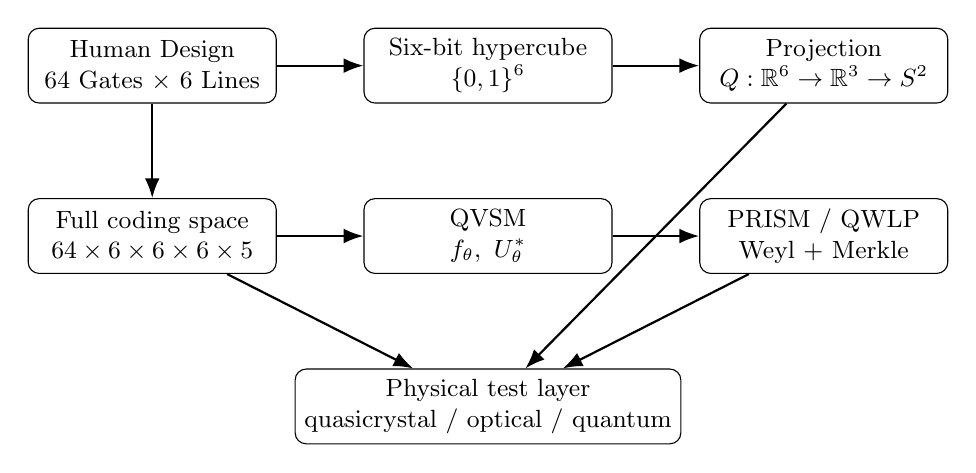
\begin{tikzpicture}[
  box/.style={draw,rounded corners,align=center,minimum width=3.15cm,minimum height=0.95cm,font=\small},
  arr/.style={-{Latex[length=2.5mm]},thick},
  node distance=1.2cm and 1.1cm]
  \node[box] (hd) {Human Design\\64 Gates $\times$ 6 Lines};
  \node[box,right=of hd] (hy) {Six-bit hypercube\\$\{0,1\}^6$};
  \node[box,right=of hy] (proj) {Projection\\$Q:\R^6\to\R^3\to S^2$};
  \node[box,below=of hd] (full) {Full coding space\\$64\times6\times6\times6\times5$};
  \node[box,right=of full] (qvsm) {QVSM\\$f_\theta,\ U_\theta^*$};
  \node[box,right=of qvsm] (audit) {PRISM / QWLP\\Weyl + Merkle};
  \node[box,below=of qvsm] (phys) {Physical test layer\\quasicrystal / optical / quantum};
  \draw[arr] (hd)--(hy);
  \draw[arr] (hy)--(proj);
  \draw[arr] (hd)--(full);
  \draw[arr] (full)--(qvsm);
  \draw[arr] (qvsm)--(audit);
  \draw[arr] (proj)--(phys);
  \draw[arr] (full)--(phys);
  \draw[arr] (audit)--(phys);
  \end{tikzpicture}
\caption{Central architecture of the proposed framework. The arrows are mathematical mappings or computational interfaces; they do not assert physical equivalence between the layers.}
\label{fig:central}
\end{figure}

% ================================================================
\section{Audit protocol and reproducibility}
\label{sec:audit}

Every numerical result should be reproducible from a versioned input, deterministic seed, software environment, and machine-readable output. The recommended project layout is shown in \cref{fig:repo} and documented in the accompanying \texttt{FIGURES.md} and audit manifests.

\subsection{Minimum audit record}

For each reported quantity, archive:
\begin{enumerate}[label=(\alph*),leftmargin=2.1em]
  \item mathematical definition;
  \item input file checksum;
  \item code commit hash;
  \item numerical precision;
  \item tolerance;
  \item observed residual;
  \item expected invariant or null model;
  \item pass/fail decision.
\end{enumerate}

For example, a pseudoinverse check can record
\begin{equation}
\varepsilon_{K^+}
=
\frac{\|K K^+ K-K\|_F}{\|K\|_F}.
\end{equation}
For orbit counts the primary invariant is an integer, so an exact combinatorial implementation is preferable to floating-point arithmetic.

\begin{figure}[t]
\centering
\safegraphic[width=0.96\linewidth]{figures/fig02_repo_pipeline.pdf}{6cm}
\caption{Planned repository/audit pipeline: source state definitions feed symbolic, geometric, QVSM and PRISM layers, each producing machine-readable results and cryptographic commitments.}
\label{fig:repo}
\end{figure}

% ================================================================
\section{Results inventory from the current project}
\label{sec:inventory}

The following table collects the current project-level results that the paper is designed to formalize. ``Reported'' means that the quantity exists in the project's computational record; it does not mean that the result has already passed independent peer review.

\begin{table}[t]
\centering
\small
\begin{tabular}{p{0.27\linewidth}p{0.19\linewidth}p{0.43\linewidth}}
\toprule
Object & Current result & Audit status \\
\midrule
Full symbolic space & $69\,120$ & Exact factorization from $(64,6,6,6,5)$. \\
Hexagram layer & $Q_6$, 64 vertices & Exact graph construction. \\
$V_{\rm Hex}\otimes T_2$ & 192 dimensions & Exact tensor-product dimension; physical interpretation open. \\
Supergolden substitution & $\psi^3-\psi^2-1=0$ & Exact algebraic definition; face-incidence implementation to be independently rerun. \\
PRISM initial cycles & $216\times320$ & Project computational record. \\
PRISM dynamic orbits & 108 orbits of length 640 & Project computational record; equivalence relation must be documented explicitly. \\
Spatial/Gram quotient & 20 classes & Project computational record. \\
QVSM & $\dim=16$, 120 epochs & Training record; independent rerun required. \\
QVSM factor accuracy & $0.96875,1,1,1,1$ & Training record; seed/metric manifest required. \\
Covariance residuals & $(0.13384,0.00177,0.00295,0.00191,0.00108)$ & Diagnostic record; interpretation limited to representation quality. \\
$K_{\rm tangent}$ & relative pseudoinverse tolerance $<10^{-16}$ claimed & Must be rerun from exact JSON block. \\
ATLAS $ZZ^*$ & 4.7$\sigma$ separable-state rejection & External experimental reference, not a result of this framework. \\
\bottomrule
\end{tabular}
\caption{Project results and their evidentiary status.}
\label{tab:inventory}
\end{table}

% ================================================================
\section{Predictions and falsification criteria}
\label{sec:predictions}

The framework should be judged by predictions that could fail.

\subsection{P1: optical geometric response}
A quasicrystalline sample prepared in a prescribed orientation should exhibit a reproducible change in a predefined observable under controlled optical excitation if the optical hypothesis is correct:
\[
\Delta O(\lambda,I,\mathbf p)\ne0.
\]

\subsection{P2: supergolden spectral signature}
A specified substitution or face-transition operator should have a Perron root equal to $\psi$ within a declared numerical tolerance, and the characteristic polynomial should contain the factor $x^3-x^2-1$.

\subsection{P3: symmetry invariants}
For a declared group action, orbit and Gram invariants should remain unchanged under the specified gauge transformations. Any discrepancy must be localized to a transformation rule, implementation or numerical tolerance.

\subsection{P4: QVSM shift covariance}
The learned operator should satisfy a held-out equivariance test,
\begin{equation}
\varepsilon_U=
\frac{\|U_\theta^* f_\theta(X)-f_\theta(\tau X)\|_2}
{\|f_\theta(\tau X)\|_2}
\ll1
\end{equation}
with a threshold fixed before evaluation.

\subsection{P5: quantum-map nontriviality}
A proposed map $X\mapsto\rho_X$ is meaningful only if it yields observables with a predictive advantage over a null model. Mere visual similarity to Bell tetrahedra, spin density matrices or particle diagrams is not sufficient.

% ================================================================
\section{Discussion}
\label{sec:discussion}

The principal conceptual result is a change of framing. The Human Design architecture is not used here as a proof of a physical theory. It is used as a discrete coordinate system with a documented internal hierarchy. This creates a precise interface to combinatorics and geometry.

The first nontrivial interface is
\[
64\rightarrow\{0,1\}^6,
\]
which embeds the 64 Gate states into a canonical hypercube. The second is a projection from six-dimensional coordinates to a three-dimensional geometric sector. The third is the factorized extension from 64 states to 69,120 symbolic states. The fourth is the lifting into learned and certifiable representations.

The quasicrystalline branch is particularly natural as a mathematical comparison because icosahedral quasicrystals are themselves routinely described by six-dimensional models cut into three-dimensional physical space \citep{VanSmaalen1991,YamamotoTakakura2003}. This is a structural analogy with precise mathematical content. Whether a physical sample realizes any of the proposed Human Design-derived operators is an experimental question.

The supergolden branch supplies a second spectral language. The root $\psi$ is not inserted because it is aesthetically close to $\phi$; it is selected by an explicit characteristic polynomial. The same principle should govern all later constants: define the matrix first, then derive its spectrum.

The quantum branch should remain the most conservative. The 2026 ATLAS result on $ZZ^*$ entanglement is significant because it demonstrates that high-energy experiments can reconstruct genuinely quantum correlation structure from decay kinematics \citep{ATLASZEntanglement2026}. But the result is logically independent of the present coding construction. A future bridge therefore has to be operational: specify the state, observable, map, uncertainty and null hypothesis.

% ================================================================
\section{Limitations}
\label{sec:limitations}

Several limitations are explicit.

First, Human Design is not an established physical theory. The manuscript therefore does not treat its symbolic claims as experimentally validated premises.

Second, the project's numerical results need an independent reproduction package with pinned dependencies, deterministic seeds, complete input arrays and exact transformation definitions. Reported hashes and orbit counts should not be treated as evidence until the corresponding files are publicly inspectable.

Third, the mapping from the 64-state hypercube to a physical quasicrystal is not unique. Many linear projections $Q$ exist, and an acceptable selection must be justified by symmetry, optimization or experimental calibration rather than visual appeal.

Fourth, a correspondence between finite combinatorial structures and quantum correlation polytopes does not establish a common physical ontology. Mathematical isomorphism, representation equivalence and physical identity are different claims.

Fifth, an optical effect in a quasicrystal, even if observed, would establish a materials response. It would not by itself validate Human Design. The scientific bridge has to specify what quantity is shared and why the same invariant is observed independently in both contexts.

% ================================================================
\section{Conclusions}
\label{sec:conclusion}

This paper defines a research program in which Human Design is treated as a discrete coding layer rather than a physical proof system. The documented 64-Gate hierarchy and its Line/Color/Tone/Base subdivision naturally define a 69,120-state product space. The 64 Gate layer has a canonical six-bit hypercube representation, enabling exact Hamming geometry and a natural complement involution. A three-dimensional projection and a $64\times3=192$ tensor-product lifting then provide a route to the project's $T_2/T_{2u}$ geometry.

A quasicrystalline cut-and-project branch supplies a mathematically established six-to-three-dimensional comparison class. A supergolden substitution adds an explicit algebraic spectral invariant, while QVSM and PRISM/QWLP provide learned and cryptographically auditable transformations. Modern $ZZ^*$ entanglement measurements supply an external experimental reference for the level of operational specificity required in a quantum claim.

The strongest version of the program is therefore not ``Human Design proves quantum physics''. It is:
\begin{equation}
\boxed{
\text{symbolic architecture}
\rightarrow
\text{explicit geometry}
\rightarrow
\text{reproducible computation}
\rightarrow
\text{certified invariants}
\rightarrow
\text{falsifiable experiment}
}
\end{equation}
Only the final experimental step can determine whether any proposed physical correspondence is more than a mathematically interesting representation.

% ================================================================
\appendix
\section{Canonical definitions}
\label{app:canonical}

\subsection{State index}
For $X=(G,L,C,T,B)$,
\[
i=((((G\,6+L)\,6+C)\,6+T)\,5+B).
\]
The inverse map is obtained successively by Euclidean division by $5$, $6$, $6$, and $6$.

\subsection{Six-bit encoding}
Let $G$ be represented by its binary expansion
\[
G=\sum_{k=0}^{5}2^k g_k,
\qquad g_k\in\{0,1\}.
\]
The choice of bit ordering must be fixed in the machine-readable manifest.

\subsection{Complement}
\[
G^c=G\oplus63.
\]
This is an involution because $63\oplus63=0$.

\subsection{Product-space shift}
\[
\tau(G,L,C,T,B)=(G+1\!\!\pmod{64},L+1\!\!\pmod6,C+1\!\!\pmod6,T+1\!\!\pmod6,B+1\!\!\pmod5).
\]

\section{Reproducible command targets}
\label{app:commands}

The repository is intended to expose deterministic targets such as:
\begin{verbatim}
python -m audit.reproduce_all --manifest data/audit/manifest.json
python -m audit.symbolic_tests
python -m geometry.hypercube64
python -m geometry.supergolden
python -m qvsm.learned_audit
python -m prism.certification
\end{verbatim}
Exact module names can be changed without changing the mathematical specification; the audit manifest is the authoritative interface.

\section{Figure registry}
\label{app:figregistry}

The planned figures and filenames are defined in the companion \texttt{FIGURES.md}. Main-text figure labels are kept stable so the raster/vector assets can be regenerated without editing the mathematical prose.

% ================================================================
\bibliographystyle{plainnat}
\bibliography{references}

\end{document}
